\documentclass[12pt]{article}
\usepackage{amsmath}
\usepackage{amssymb}
\usepackage{hyperref}
\usepackage{graphicx}
\usepackage[center]{titlesec}
\usepackage[utf8]{inputenc}
\usepackage[english]{babel}
\newcommand{\R}{\mathbb{R}}

\title{Algorithmic Operation Research \\ Homework 3}
\date{8-11-2019}
\author{Theodora Panagea - 1115201400135 \\ Anna-Aikaterini Kavvada - 1115201500050}

\begin{document}
	\maketitle{}
  	\pagenumbering{arabic}
  	\newpage
  	
%---------Choosing paths in a network----------
\section{Choosing paths in a network}
A communication network aims to create a liaison between two devices or more, a \textbf{receiver} and a \textbf{transmitter}. It consists of the two aforementioned parties and all in-between devices, called nodes, which are connected with \textbf{communication links}. Let's consider a set $N$ that consists of all the nodes, and a set $A$, which includes all links available in our network. For example, if we take the nodes $i,j \in N$, then the ordered \textbf{pair} $(i,j) \in A$. We assume that the link $(i,j)$ can carry up to $u_{ij}$ bits per second. Along that link, a positive charge $c_{ij}$ per bit is transmitted. Each node $k$ generates data, at the rate of $b^{kl}$ bits per second, that have to be transmitted to node $l$, either through a direct link $(k,l)$, or by tracing a \textbf{sequence of links}.  

\subsection*{Problem}
The problem we have to face is to choose the right path, along which all data reach their intended destinations, while minimizing the cost. \\
\textbf{Note:} Data with the same origin and destination, can be split and transmitted along different paths. \par

 \subsection*{Formulating as a Linear Programming Problem}
We have $x_{ij}^{kl}$	which indicates the amount of data with origin $k$ and destination $l$, that traverse link $(i,j)$. Let
$$b_i^{kl} = 
\begin{cases} 
      b^{kl},     \text{\quad  if }   i = k \\
      -b^{kl},    \text{ if }  i = l \\  
      0,            \text{ \quad otherwise}
   \end{cases}$$
Therefore, $b_i^{kl}$ is the net inflow at node $i$, with origin $k$ and destination $l$, from outside the network. We need to construct a function, which represents the cost we need to minimize. The cost will be the sum of all possible combinations of origin, destination and traverse links, and for each combination, the cost is the charge $c_{ij}$ per bit per second of the traverse link $(i,j)$, multiplied by $x_{ij}^{kl}$, the amount of data needed to be transmitted from $k$ to $l$, through that link.\\
 So, our main \textbf{goal} is:
\begin{equation*}
\text{minimize} \quad \sum_{(i,j) \in A} \sum_{k=1}^{n} \sum_{l=1}^{n}{c_{ij}x_{ij}^{kl}} \quad \qquad \qquad \qquad \qquad \qquad \qquad \quad
\end{equation*}

\begin{equation*}
 \text{subject to} \sum_{\lbrace j| (i,j) \in A\rbrace}{x_{ij}^{kl}} - \sum_{\lbrace j| (j,i) \in A\rbrace}x_{ji}^{kl} = b_i^{kl}, \qquad i,k,l=1,\ldots,n 
\end{equation*}

\begin{equation*}
\sum_{k=1}^n\sum_{l=1}^n x_{ij}^{kl} \leqslant u_{ij}, \qquad  \qquad \quad (i,j) \in A
\end{equation*}

\begin{equation*}
x_{ji}^{kl} \leqslant 0, \qquad (i,j) \in A \quad  k,l = 1,\ldots, n
\end{equation*}
The first constraint is a flow conservation constraint at node $i$ for data with origin $k$ and destination $l$. The expression 
$$\sum_{\lbrace j| (i,j) \in A\rbrace}{x_{ij}^{kl}}$$ represents the amount of data with origin $k$ and destination $l$, that \textbf{leave} node $i$ along some link. The expression $$\sum_{\lbrace j| (j,i) \in A\rbrace}x_{ji}^{kl}$$ represents the amount of data with the same origin and destination as the above, but \textbf{enter} node $i$ along some link. Finally, $b_i^{kl}$ is the net amount of such data that enter node $i$ from outside the network. The second constraint function expresses the requirement that the total traffic through a link $(i,j)$ cannot exceed the link's capacity.  \\
This problem is a \textbf{multicommodity flow} problem. Routing and wavelength assignment (RWA) in optical burst switching of Optical Network would be approached via multicommodity flow formulas.
\newpage
\subsection*{Extension}
If we consider the network as a graph, where a link is an \textbf{edge} between two nodes, with weight equal to the positive charge it produces, then all we have to do is to find the shortest path between two nodes, while also checking that each edge can carry the asked amount of bits. 
There are several algorithms for these problems, such as \textbf{Dijkstra}, which is already in use, in terms of routing. \\
A small example is shown below, where a network is represented as a graph, and the pair above each edge, shows its cost and its capacity.
\newline \newline
\begin{figure}[h!]
  \begin{center}
  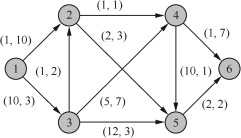
\includegraphics[width=10cm]{netgraph.jpg}
  \end{center}
\end{figure}
\newpage

%-------Pattern Classification-------------------
\section{Pattern Classification}
{Let's consider \textbf{$m$} examples of \textbf{objects} and for each one, a description of its features in terms of an \textit{n-dimensional} \textbf{vector}. Thus, the $i$-th object is described by the vector $a_i$.\par
For the above case, we set 2 \textit{classes} of objects. For each example, we know the class it belongs to, thus considering the above set of data as the test set we will use for a classifier.\par
\subsection*{Goal}
At this point our goal, is to design a classifier which, given a new object, suppose \textbf{$k$}, that does not belong to the test set, will be able to decide in which class \textbf{$k$} belongs, regarding its features stored in vector $a_k$.\par
\subsection*{What Is A Linear Classifier?}
\textbf{\textit{Definition:}} An $n$-dimensional vector $x$, which is considered the basis of a \textit{linear combination} of the different features of an object, and a \textit{scalar} $x_{n+1}$, that defines the range of each class taking in consideration all the features available.\\
\textbf{\textit{Operation:}} Given a new object $k$, with feature vector $a_k$, the classifier declares it to be an object of the first class, if the following constraint is met:
$$\bullet \quad \alpha'x \geq x_{n+1}$$
Otherwise, in case the constraint below is met, the item belongs to the second class of objects:
$$\bullet \quad \alpha'x < x_{n+1}$$
\newpage
\subsection*{Designing A Linear Classifier}
So, how do we design a good linear classifier, using the available examples/test set? 
A reasonable starting point for that, is the requirement for the classifier to give the correct answer, meaning to classify the available example in the proper class. Let $S$ be the set of examples of the first class. We are then looking for some $x$ and $x_{n+1}$ that satisfy the constraints
$$\bullet \quad \alpha'_ix \geq x_{n+1} \quad i \in S$$
$$\bullet \quad \alpha'_ix < x_{n+1} \quad i \notin S$$
\textbf{Note:} the second set of constraints involves a strict inequality and is not quite of the form arising in linear programming. 
\textbf{Resolve Issue:} We can resolve this issue by observing that if some choice of $x$ and $x_{n+1}$ satisfies all of the above constraints, then there exists some other choice if we multiply $x$ and $x_{n+1}$ by a suitably large scalar, that satisfies the below constraints:
$$\bullet \quad \alpha'_ix \geq x_{n+1} \quad i \in S$$
$$\bullet \quad \alpha'_ix \leq x_{n+1} \quad i \notin S$$
It is like curving a convex hull around the original scalar of the second class, in order to satisfy the demands of a linear program.\par
\newpage
\subsection*{Conclusion}
We conclude that the search for a linear classifier which is consistent with all available examples is a problem of finding a set of values applicable for the decision variable - the second class in this case. This set satisfies the entire constraints provided in the optimization problem (\textit{feasible solution}).The feasible region of the optimization problem is defined by all the set of the feasible solutions. In most of the optimization algorithms first, an attempt is made to find the feasible solution and then another attempt is made to locate another feasible solution which will improve the objective function value. The process of making an attempt to search the improving feasible solution goes on until there are no chances of further improvement or any other criteria of stopping this process is met.
\begin{figure}[h!]
  \begin{center}
  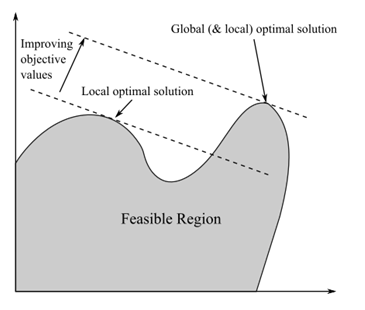
\includegraphics[width=50mm]{FeasibleSolution.png}
  \caption{}
  \label{figure}
  \end{center}
\end{figure}
\newpage
\subsection*{Extension}
\par  Nowadays, we see many applications of Linear Classifiers in Computer Science (i.e. Data Mining, Machine Learning).Below follow two widely known competitive algorithms used to solve Pattern Classification Problems:
\begin{itemize}
    \item \textbf{Multinomial Naive Bayes:}With a multinomial event model, samples (feature vectors) represent the frequencies with which certain events have been generated by a multinomial $(p_1, \dots, p_n)$ where $p_{i}$ is the probability that event $i$ occurs (or $K$ such multinomials in the multiclass case). A feature vector ${\mathbf  {x}}=(x_{1},\dots ,x_{n})$ is then a histogram, with $x_{i}$ counting the number of times event i was observed in a particular instance. This is the event model typically used for document classification, with events representing the occurrence of a word in a single document (see bag of words assumption). The likelihood of observing a histogram $x$ is given by

$$ p(\mathbf {x} \mid C_{k})={\frac {(\sum _{i}x_{i})!}{\prod _{i}x_{i}!}}\prod _{i}{p_{ki}}^{x_{i}}$$
The multinomial naive Bayes classifier becomes a linear classifier when expressed in $log$-space:

$${\begin{aligned}\log p(C_{k}\mid \mathbf {x} )&\varpropto \log \left(p(C_{k})\prod _{i=1}^{n}{p_{ki}}^{x_{i}}\right)\\&=\log p(C_{k})+\sum _{i=1}^{n}x_{i}\cdot \log p_{ki}\\&=b+\mathbf {w} _{k}^{\top }\mathbf {x} \end{aligned}}$$
where $b=\log p(C_{k})$ and $w_{{ki}}=\log p_{{ki}}$.
    \item \textbf{SVM-Support Vector Machine:}We are given a training dataset of $n$ points of the form
    $$ ({\vec {x}}_{1},y_{1}),\ldots ,({\vec {x}}_{n},y_{n}),$$ 
    where the $y_{i}$ are either $1$ or $-1$, each indicating the class to which the point ${\vec {x}}_{i}$ belongs. Each ${\vec {x}}_{i}$ is a $p$-dimensional real vector. We want to find the "maximum-margin hyperplane" that divides the group of points ${\vec {x}}_{i}$ for which $ y_{i}=1$ from the group of points for which $y_{i}=-1$, which is defined so that the distance between the hyperplane and the nearest point ${\vec {x}}_{i}$ from either group is maximized.\par
    Any hyperplane can be written as the set of points ${\vec {x}}$ satisfying
    $${\vec {w}}\dot {\vec {x}}-b=0,$$
    where ${\vec {w}}$ is the (not necessarily normalized) normal vector to the hyperplane. This is much like Hesse normal form, except that ${\vec {w}}$ is not necessarily a unit vector. The parameter ${\frac {b}{\|{\vec {w}}\|}}$ determines the offset of the hyperplane from the origin along the normal vector ${\vec {w}}$.
    \begin{figure}[h!]
      \begin{center}
      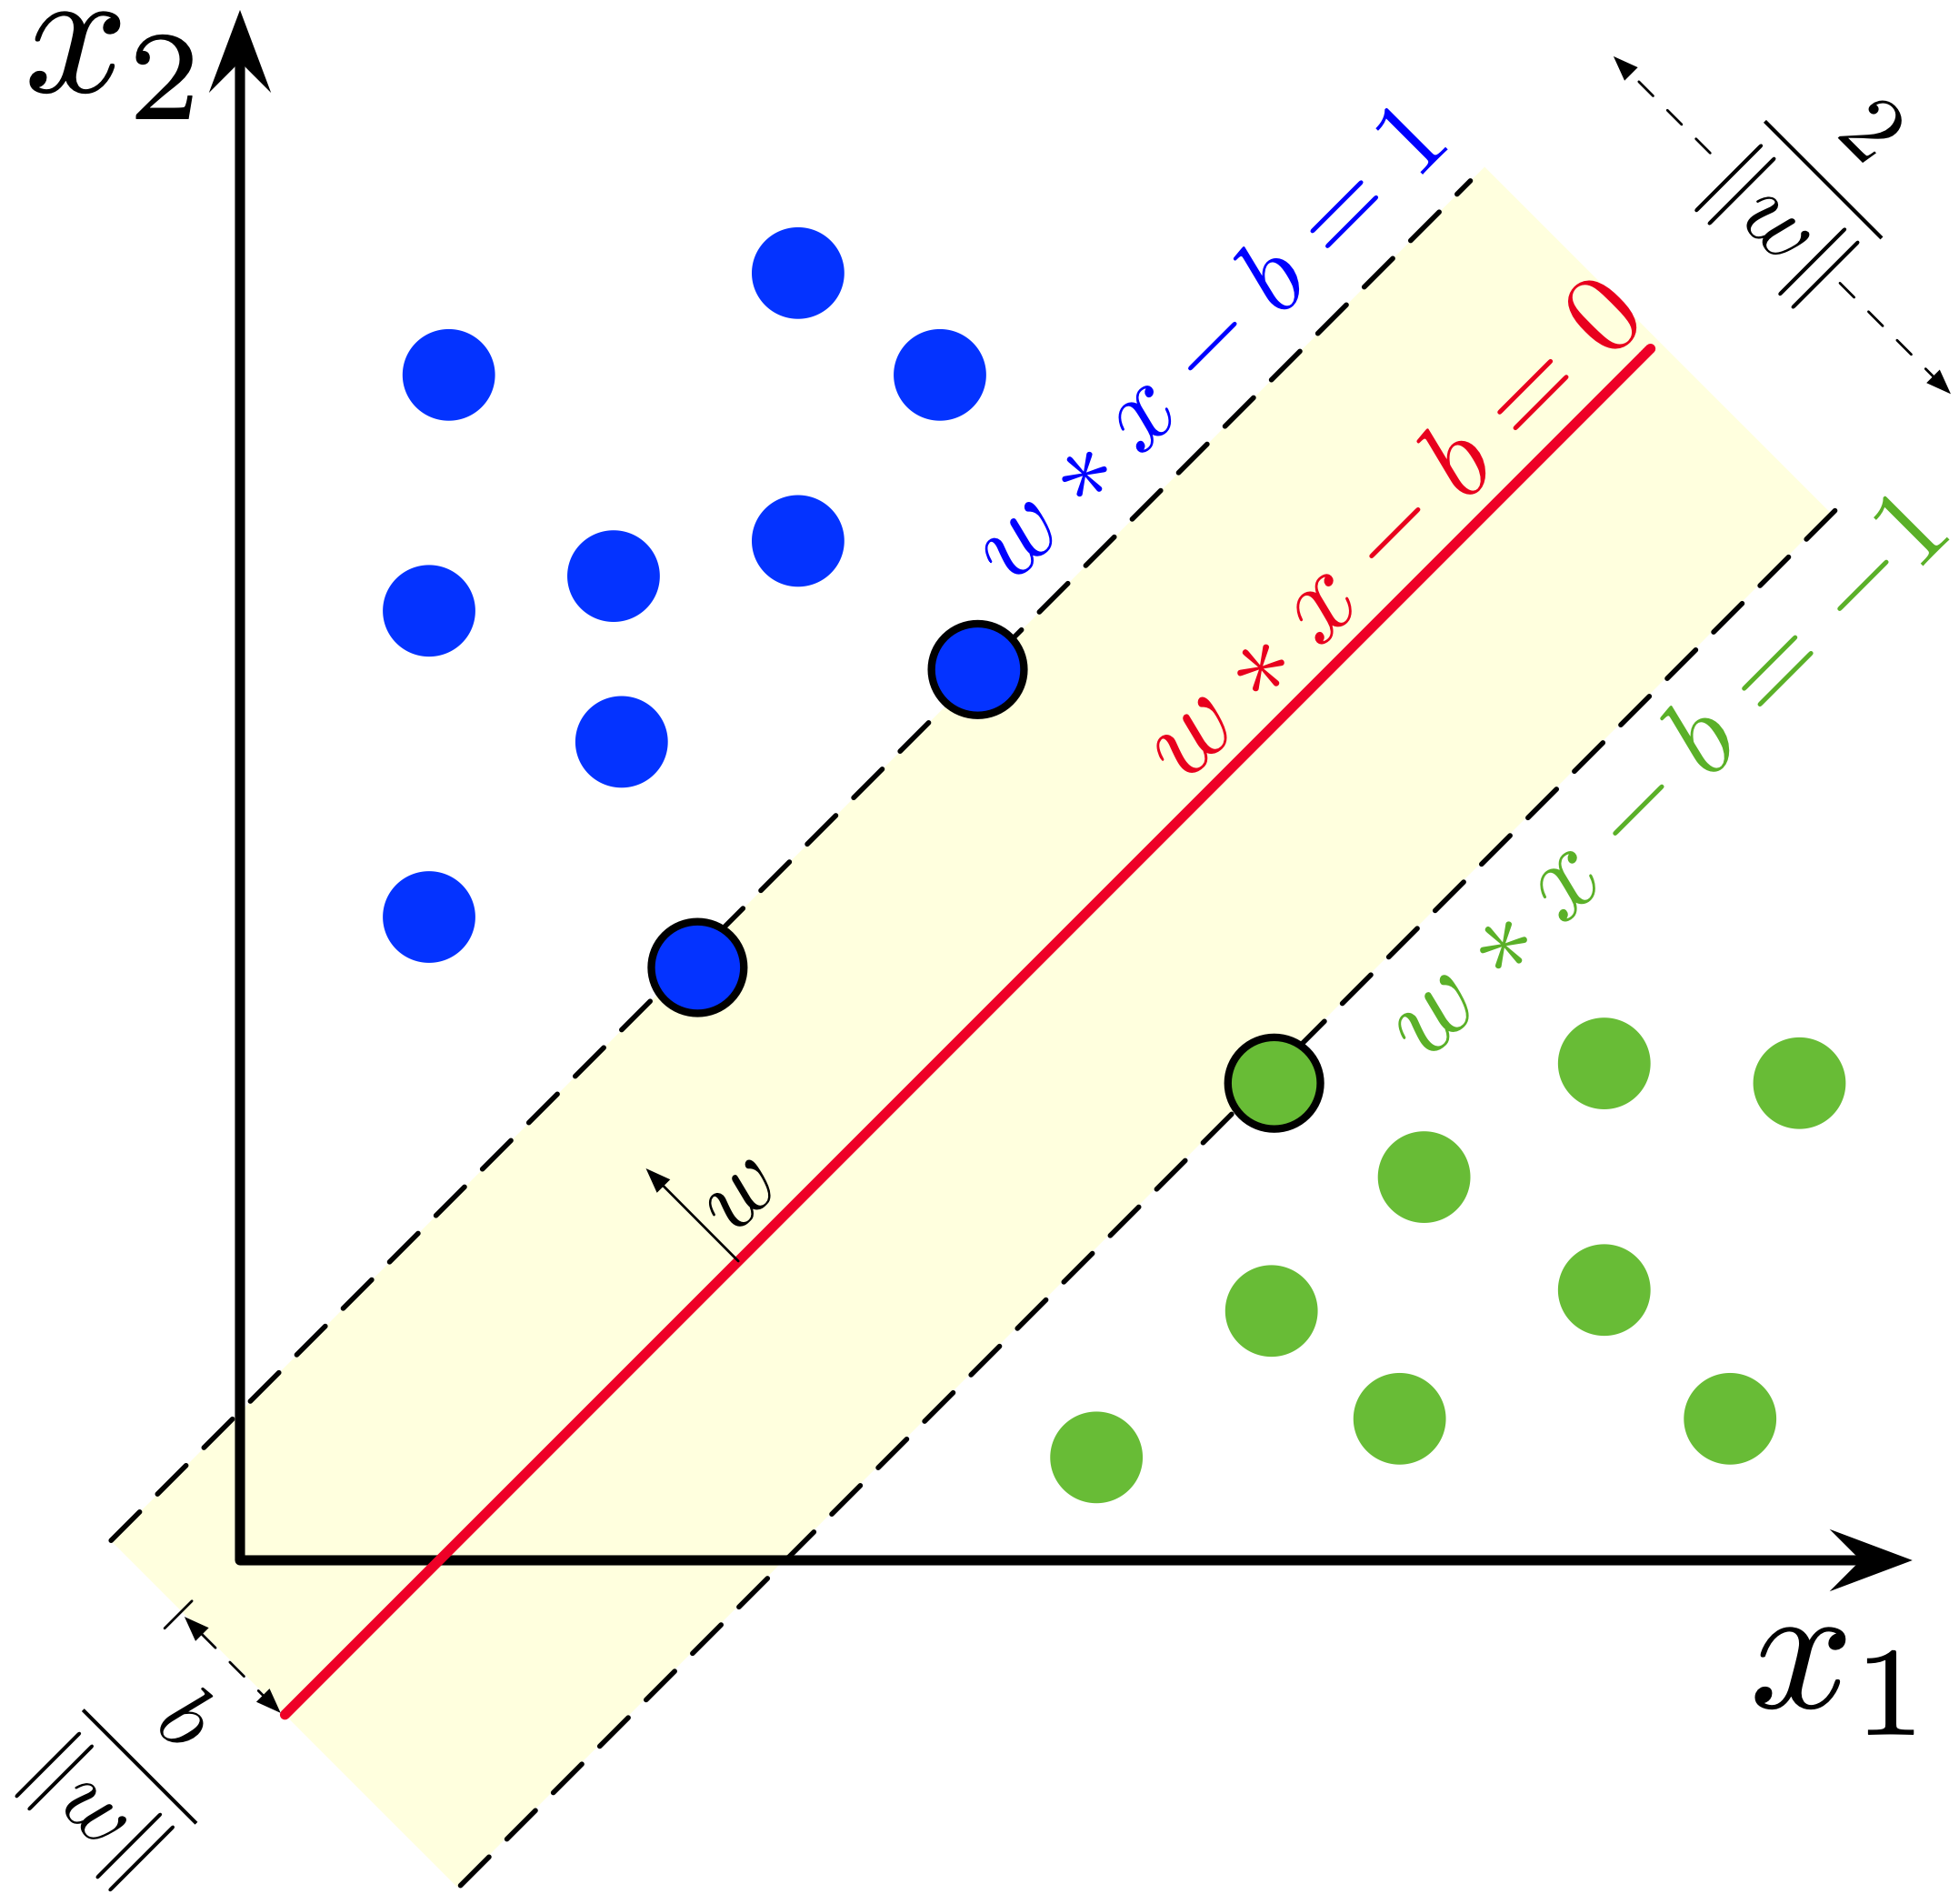
\includegraphics[width=50mm]{SVM_margin.png}
      \caption{Maximum-margin hyperplane and margins for an SVM trained with samples from two classes. Samples on the margin are called the support vectors.}
      \label{fig:}
      \end{center}
    \end{figure}
\end{itemize}
\textbf{Hesse normal form:} it is an equation used in analytic geometry, and describes a line in $\mathbb {R} ^{2}$ or a plane in Euclidean space $\mathbb {R} ^{3}$ or a hyperplane in higher dimensions.It is primarily used for calculating distances.\\
It is written in vector notation as
$${\vec  r}\cdot {\vec  n}_{0}-d=0.$$
}
 \end{document}